\pagebreak
\chapter{Continuous Integration}
%Dieses Kapitel beschäftigt sich mit einem der beiden Hauptthemen, nämlich Continuous Integration. 
Zunächst nähert sich diese Arbeit dem Thema durch eine genaue Begriffsbestimmung, wobei auch eine Abgrenzung zu anderen, ähnlichen Begriffen eine wichtige Rolle spielt. Im weiteren Verlauf sollen dann noch der grundsätzliche Ablauf sowie die Gründe zum Einsatz dieser Methodik näher beleuchtet werden.\\
\section{Begriffsklärung und Abgrenzung zu anderen Begriffen}
Den Einstieg soll eine kurze Beschreibung von Martin Fowler bilden, er gilt als der geistige Vater von Continuous Integration und wird mit diesem Artikel in vielen anderen Abhandlungen zu dem Thema zitiert:
\begin{center}
	\textit{
	Continuous Integration is a software development practice where members of a team integrate their work frequently, usually each person integrates at least daily - leading to multiple integrations per day. Each integration is verified by an automated build (including test) to detect integration errors as quickly as possible}\\ \cite{fowler-CI}
\end{center}
Es geht hier also um das kollaborative Arbeiten in einem Team, insbesondere das Integrieren von Code in eine gemeinsame Code-Basis. Das heißt ferner, dass es eine Methodik ist, die für einen einzelnen Entwickler kaum Bedeutung hat. Das ist auch einleuchtend, denn seinen eigenen Code in eben diesen zu integrieren, geschieht automatisch durch seine Änderungen. \\
Außerdem sollte die Integration sehr oft passieren, am besten mehrmals täglich. Dies ist ein sinnvolles Vorhaben, da die Wahrscheinlichkeit auf eine sehr komplexe Integration steigt, je länger man damit wartet, denn dann wird aus dem Integrieren einer eigentlich kleinen Änderung ein umfassender Mehraufwand durch das Mergen\footnote{Mergen bezeichnet das Vergleichen mehrerer Änderungen an einer Quelldatei und das Zusammenführen ("`mergen"') dieser Änderungen. (Diese Formulierung stammt vom Autor, und ist nicht durch Literatur hinterlegt)} dieser Konflikte. Ein solcher Konflikt könnte zum Beispiel eine Änderung sein, die dieselbe Code Stelle auf zwei Branches unterschiedlich geändert hat.\footnote{Dieser Konflikt tritt im Alltag des Autors als Build- und Configuration Manager des öfteren auf und ist hier nicht durch Literatur hinterlegt} \\
Der dritte Teil der vorliegenden Beschreibung geht darauf ein, wie man den Nachweis erbringen kann, dass die Integration erfolgreich war. Dafür soll es automatisierte (und dadurch auch standardisierte) Builds geben. Diese Builds erzeugen zunächst aus dem menschenlesbaren Code den von Maschinen ausführbaren Code, sowie dazugehörige Tests in verschiedenem Detailgrad. Martin Fowler gibt in seiner Beschreibung auch an, dass die Tests mit zu diesen automatisierten Builds gehören. Hierbei muss man auf eine sinnvolle Testtiefe achten. Wenn man die Test-Pyramide\footnote{Dabei handelt es sich um eine Darstellung der unterschiedlichen Testtypen in hierarchischer Form, wobei von unten nach oben die Geschwindigkeit abnimmt und die Kosten zunehmen. Vgl.:\cite{fowler-Testpyramid}} zu Rate zieht, gibt es neben UnitTests auch solche, die das Zusammenspiel mehrerer Komponenten testen. Dies muss jedoch durch höheren zeitlichen Aufwand erkauft werden. Deshalb muss darauf geachtet werden, dass alle Tests fertig sind, bevor der nächste Entwickler sein Änderungen in die Code-Basis integriert. Es kann vorteilhaft sein, wenn man während des Check-In Builds nur Unittests ausführt, und in einem möglicherweise nur einmal am Tag laufenden Build dann auch umfangreichere Test wie Komponententests, Integrationstests oder Tests auf der installierten Applikation, sogenannte Smoketests, ausführt.\\
Um diese Beschreibung der Kernpunkte von Continuous Integration auf eine breitere Basis zu stellen, soll hier noch eine zweite Quelle genutzt werden, um von einem anderen Blickwinkel auf das Thema zu blicken.
\begin{center}
	\textit{
The practice of continuous integration represents a fundamental shift\\ in the process of building software. It takes integration, commonly\\
an infrequent and painful exercise, and makes it a simple, core part\\ of a developer’s daily activities. Integrating continuously makes\\ integration a part of the natural rhythm of coding, an integral part\\ of the test-code-refactor cycle. Continuous integration is about\\ progressing steadily forward by taking small steps.}\\ \cite{10.1007/978-3-540-24853-8_8}
\end{center}
Der Autor dieses Konferenzbeitrags ist R. Owen Rogers. Er arbeitete zu dieser Zeit bei Thoughtworks, derselben Firma, bei der auch Martin Fowler arbeitet. Das Zitat stammt von einer Konferenz aus dem Jahr 2004, also zeitlich zwischen der initialen Version des Artikels über Continuous Integration (CI) von Martin Fowler und seiner aktuellen Version aus dem Jahr 2006.\\
Es wird dabei der Fokus eher auf die Auswirkungen von Continuous Integration auf die Softwareentwicklung und den Einfluss auf die Qualität von Software gelegt. Rogers geht vor allem darauf ein, dass das häufige Integrieren der zentrale Teil dieses Konzepts ist. Das deckt sich mit der oben vorgestellten Sichtweise von Martin Fowler. Des weiteren setzt er den Ansatz in den Kontext von "`test-code-refactor"', und geht damit auch auf einen anderen bereits vorgestellten Aspekt ein, nämlich das Überprüfen des Erfolgs der Integration. 
Hier wird im Gegensatz zu Fowler nicht explizit auf den Team-Aspekt eingegangen. Dieser Gesichtspunkt ist eher implizit enthalten.\\
Die Sichtweise von R. Owen Rogers deckt sich damit mit der von Martin Fowler, er beleuchtet das Thema einfach nur aus einem anderen, eher anwendungsbezogenen Blickwinkel. Das ist auch nachvollziehbar, da es sich hier nicht um eine theoretische Abhandlung handelt, sondern einen Konferenzbeitrag, der an Anwender dieser Technik gerichtet war.\\

Zusammenfassend bleibt zu sagen, dass mit Continuous Integration die Zusammenarbeit eines Entwicklerteams an einer gemeinsamen Code-Basis verbessert werden soll. Dies soll durch kontinuierliches Zusammenführen der Änderungen aller Beteiligten und das automatisierte Prüfen des Ergebnisses geschehen.
\subsection*{Abgrenzung zu anderen Begriffen}
Es gibt einige Begriffe, die Continuous Integration sehr ähnlich sind. Im Folgenden soll genauer umrissen werden, worin der Unterschied und eventuelle Gemeinsamkeiten liegen.
\begin{itemize}
	\item\textbf{Continuous Delivery}\label{Continuous Delivery}\\
	Eine zusammenfassende Definition von Martin Fowler:
\begin{center}
	\textit{
	You achieve continuous delivery by continuously integrating the \\software done by the development team, building executables, and\\ running automated tests on those executables to detect problems. \\Furthermore you push the executables into increasingly production-like \\environments to ensure the software will work in production. To do \\this you use a DeploymentPipeline.}\\ \cite{fowler-CD}
\end{center}
	Bei Continuous Delivery (CD) wird der Gedanke von Continuous Integration aufgegriffen, und weiterentwickelt. Während Continuous Integration sich komplett in der Entwicklung bewegt, umfasst Continuous Delivery auch Schritte bis hin zum Kunden. Es werden weitere Schritte wie das Paketieren als Deliverable (z.B. Erstellen eines Setups) und das Deployment (z.B. Bereitstellen als Download oder Einstellen in einen AppStore) betrachtet. Das Ziel dessen ist, dass das Ergebnis der Entwicklung zum geplanten Auslieferungszeitpunkt bereit ist für den Kunden.\\
	\item\textbf{Continuous Deployment}\label{Continuous Deployment}\\
	Hier beziehe ich mich auf den Abstract eines Konferenzbeitrages von Helena Holmström Olsson
	\begin{center}
		\textit{
		The concept of continuous deployment, i.e. the ability to deliver software functionality frequently to customers \textelp{}}\\
		\cite{olsson2012climbing}
	\end{center}
	Continuous Deployment bringt das CI-Konzept noch einen Schritt weiter als Continuous Delivery. Nicht nur wird hier wie bei Continuous Delivery in "`Production-like"' Umgebungen installiert, sondern sehr häufig (potentiell mit jedem Build) in die Produktion gegeben. Der Unterschied zu Continuous Delivery wirkt zunächst nur marginal, aber prinzipiell kann man sagen, dass bei Continuous Delivery festgelegt wird, wann man in die Produktion geht, und bei Continuous Deployment dies laufend passiert. \cite{scrum-overview-ci-cd}. Das heißt aber auch, dass dieses Konzept das am weitesten automatisierte ist, mit allen Vor- und Nachteilen.
	
	
\end{itemize}

In \autoref{fig:ci-cd-image-1024x384} sind die vorgestellten Begriffe in Kontext zueinander gesetzt, wobei zusätzlich noch Agile Development und DevOps genannt sind, die aber hier nicht näher erläutert werden.

\begin{figure}[h]
  \centering
  \fbox{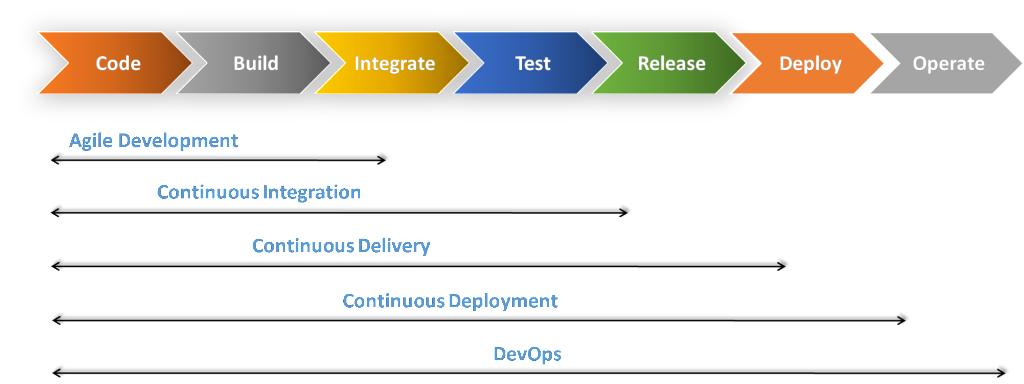
\includegraphics[width=\textwidth]{./Images/ci-cd-image-1024x384.png}}
  \caption{Einordnung von CI und ähnlicher Begriffe \cite{Begriff-Overview}}\label{fig:ci-cd-image-1024x384}
\end{figure}

\section{Ablauf von Continuous Integration}
In diesem Kapitel beziehe ich mich auf den Ablauf von CI wie er im Unterabschnitt "`Building a Feature with Continuous Integration"' von \cite{fowler-CI} beschrieben wird.
Da in der Beschreibung von CI die Rede von der Integration von Codeänderungen ist, muss es auch eine gemeinsame Basis geben, in die diese Änderungen einfließen. Eine solche gemeinsame Basis ist ein sogenanntes Source-Control-Management-System (SCM). Dabei handelt es sich um ein System, in dem Änderungen an einer Datei, oder der Struktur der Dateien, nachvollziehbar gemacht werden, und man verschiedene Stände abrufen kann (vgl. \cite{fowler-CI}). 
Es löst auch viele andere Probleme, die bei der Zusammenarbeit entstehen können, wie das gegenseitige Überschreiben von Änderungen. \\
Verschiedene Konzepte existieren hierzu, die entweder eine zentrale Stelle, an der alle Dateien inklusive Historie verwaltet werden, haben, oder verteilte Systeme, bei der es keine ausgezeichnete zentrale Instanz gibt.\\
In \autoref{fig:Schema-aufbau} ist der schematische Ablauf von CI zu sehen, wobei auf jeden der Schritte im Folgenden genauer eingegangen wird. Bidirektionale Pfeile stellen dabei eine Aktion dar, die einer Art Request-Response entsprechen, wie z.B. Dateien aus dem SCM holen entspricht Aktion starten und in der Rückrichtung Dateien erhalten.
\begin{figure}[h]
  \centering
  \fbox{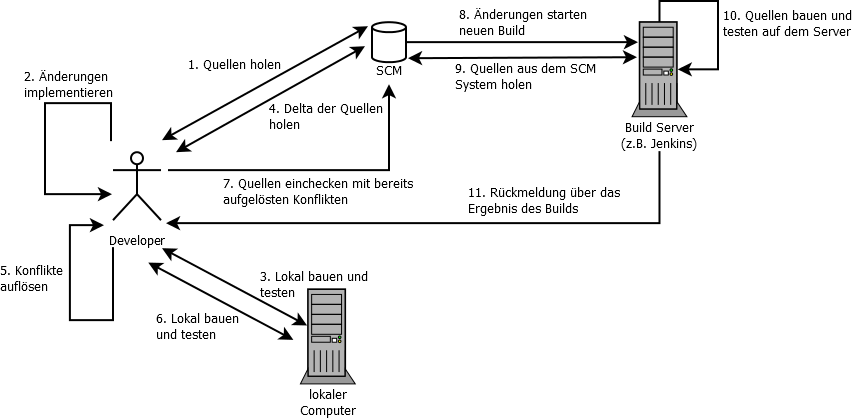
\includegraphics[width=\textwidth]{./Images/Schema-aufbau.png}}
  \caption{Schematischer Ablauf von CI}\label{fig:Schema-aufbau}
\end{figure}
\begin{enumerate}
	\item \textbf{Quellen holen}\\% 1
		Die Arbeit des Entwicklers basiert auf dem aktuellen Stand der Quellen aus dem SCM. Deshalb holt er sich zunächst diesen auf seinen lokalen Computer, um seine Arbeit zu beginnen.
		\item \textbf{Änderungen implementieren}\\% 2
		Der Entwickler folgt diesem Prozess aus einem bestimmten Grund, nämlich entweder um ein neues Feature zu implementieren oder bekannte Fehler in der Software zu beheben. Denkbar ist auch, dass er hier fehlende Tests nachliefert oder fehlschlagende Tests in Ordnung bringt. Dies geschieht in diesem Schritt. Der Entwickler führt die ihm übertragenen Aufgaben aus. Dabei wird bei CI besonderer Wert auf Tests gelegt. Dieser sehr hohe Stellenwert von Tests ist mittlerweile zum Quasi-Standard in der Softwareentwicklung geworden und folgt dem schematischen Aufbau der Testpyramide, wie sie in (\cite{fowler-Testpyramid}) beschrieben wird.
		\item \textbf{Lokal bauen und testen}\\% 3
		Der vorhergehende Schritt hat sich komplett auf das Implementieren und Ändern von Code und Tests beschränkt. Diese müssen auch noch auf Fehlerfreiheit überprüft werden, bevor man sie in das SCM einfügt. Die erste Kontrollinstanz ist nun der automatisierte Build auf der Entwicklermaschine. Darunter versteht man das Kompilieren und Linken\footnote{Dabei werden einzelne Objekt-Dateien zu Bibliotheken oder ausführbaren Dateien zusammengeführt} der Quellen, sowie das Ausführen der zuvor geschriebenen automatisierten Tests. Hierbei beschränkt man sich zumeist auf UnitTests.
		\item \textbf{Delta der Quellen holen}\\% 4
		Während ein Entwickler seinen Auftrag ausgeführt hat, könnten einige seiner Kollegen bereits ihre Arbeit vollendet haben. Deshalb sollte er nun den aktuellen ("`top-level"') Stand holen, weil es sonst zum Beispiel passieren könnte, dass Änderungen überschrieben werden oder Konflikte beim Hinzufügen zum SCM entstehen, die nicht automatisch aufgelöst werden können.
		\item \textbf{Konflikte auflösen}\\% 5
		Falls der Entwickler nun in die Situation gekommen ist, dass seine lokalen Änderungen mit Änderungen, die bereits im SCM sind, in Konflikt stehen, so muss er diese manuell auflösen. Es gibt einige Konflikte, die grundsätzlich auch toolunterstützt automatisch auflösbar sind (z.B. Änderung an derselben Datei, aber in unterschiedlichen Zeilen), jedoch können manche Konflikte nur durch manuellen Eingriff eines Menschen aufgelöst werden. Dies gilt vor allem, wenn der semantische Zusammenhang der Änderungen eine wichtige Rolle spielt.
		\item \textbf{Lokal bauen und testen}\\% 6
		Der Entwickler muss durch nochmaliges Bauen überprüfen, ob seine Änderungen noch funktionieren und alle Tests weiterhin fehlerfrei sind. Dies betrifft nun nicht nur seinen eigenen Code, sondern auch den der anderen Entwickler. Es ist denkbar, dass seine Änderungen Auswirkungen an den Code-Stellen oder Tests hat, die in der Zwischenzeit entstanden sind. Dabei ist er selbst in der Verantwortung, dass der Code-Stand, den er später dem SCM hinzufügen möchte, funktioniert. 
		\item \textbf{Quellen einchecken mit bereits aufgelösten Konflikten}\\% 7
		Nachdem lokal der Code erfolgreich kompilierbar ist, sowie alle (Unit-)Tests fehlerfrei sind, kann der Entwickler seine Änderungen dem SCM hinzufügen.
		\item \textbf{Änderungen starten neuen Build}\\% 8
		Je nach SCM und Buildserver-Kombination gibt es mehrere denkbare Ansätze automatisiert nach jedem Check-In von Code einen Build zu triggern. Diese basieren sehr häufig auf dem Observer-Pattern\footnote{Ziel des Observer Patterns ist es eine sog. one-to-many Beziehung zwischen Objekten zu definieren, so dass eine Statusänderung eines Objektes all davon abhängigen Objekte benachrichtigt, bzw. automatisch ändert. vgl. auch \cite{hannemann2002design}} entweder mit Push-Notification (Alle Subscriber werden bei einer Änderung benachrichtigt) oder Pull-Notification (Regelmäßiges Nachfragen durch die Subscriber, ob sich etwas geändert hat). Egal welche der Methoden zum Einsatz kommt, nach dem Hinzufügen der Änderungen wird ein Build gestartet.
		\item \textbf{Quellen aus dem SCM System holen}\\% 9
		Der Buildserver wurde bisher nur benachrichtigt, es ist aber noch kein Inhalt übertragen worden. Das geschieht in diesem Schritt. Der Einfachheit halber wurde in \autoref{fig:Schema-aufbau} nur ein einziger Buildserver eingefügt. Prinzipiell gibt es sehr häufig eine Orchestrierungs-Instanz und mehrere Buildserver. Diese zentrale Instanz koordiniert dabei die Aufgaben und die Server führen diese aus. Im vorliegenden Schaubild ist sowohl die koordinierende Instanz als auch die ausführende auf demselben Server. Die Übertragung der Quellen findet auf die ausführende Instanz statt, da diese auch den Code kompiliert und testet.
		\item \textbf{Quellen bauen und testen auf dem Server}\\% 10
		Anschließend wird, genau wie auch auf dem lokalen Rechner des Entwicklers, der Code gebaut und getestet. Der große Vorteil gegenüber den Entwicklerrechnern ist, dass es sich um eine klar definierte Instanz handelt. Entwicklerrechner sind sehr heterogen vom Aufbau, da im Laufe der Zeit immer mehr "`HilfsTools"', die das Arbeiten erleichtern, oder Bibliotheken hinzukommen. Der Buildserver ist anders, denn er verfügt über eine genau festgelegte Zusammenstellung von installierten Programmen und Bibliotheken, die zum Erstellen der Kompilate und dem Testen, benutzt werden können. Hier fällt zum ersten Mal auf, falls der Entwickler sich auf etwas verlässt, das nur auf seiner Maschine vorhanden ist. Dazu zählen zum Beispiel neue Kompilate. Wenn die Source Dateien nicht explizit in das SCM eingefügt wurden bzw. die Anweisungen zum Erstellen des Kompilats aus diesen Dateien fehlen, funktioniert zwar der lokale Build, aber nicht der Server Build. Dies ist das zentrale Quality Gate im CI Prozess und aufgrund des automatisierten Prozesses und der klar definierten Umgebung die Komponente, in deren Ergebnis das größte Vertrauen zu setzen ist.
		\item \textbf{Rückmeldung über das Ergebnis des Build}\\% 11
		Nachdem der Build fertig ist, muss der Entwickler auch noch auf irgendeine Art und Weise Kenntnis vom Ergebnis erlangen. Entweder wird es auf einer Webseite veröffentlicht, oder er bekommt direkt eine Benachrichtigung mit dem Ergebnis, oder eine Kombination aus beidem. Dies ist wichtig, denn abhängig vom Ergebnis des Builds hat dies Auswirkungen auf die weitere Arbeit. Der schlechtere Fall ist, dass der Build nicht funktioniert hat. Das bedeutet, dass alle anderen Entwickler, die sich auf diesen Build stützen müssen, blockiert sind in ihrer Arbeit. Dies hat zur Folge, dass so schnell wie möglich der Grund gefunden werden muss und dieses Problem behoben wird. Potentielle Lösung wäre auch, die Änderungen im SCM rückgängig zu machen, damit die anderen Entwickler vorerst ungestört weiter arbeiten können. Im guten Fall, in dem der Build erfolgreich war, signalisiert die Benachrichtigung, dass der Entwickler sich nun der nächsten Aufgabe widmen kann.
\end{enumerate}
%Ein Entwickler nimmt sich nun den aktuellen Stand aus diesem SCM, und führt seine Arbeit aus. Dabei wird bei CI besonders Wert auf Tests gelegt. Dies ist mittlerweile zum Quasistandard in der Sotwareentwicklung geworden, und folgt vom schematischen Aufbau her der Testpyramide, wie sie in (\cite{fowler-Testpyramid}) beschrieben wird.\\
%Die erste Kontrollinstanz ist nun der automatisierte Build auf der Entwicklermaschine. Darunter versteht man das Kompilieren und Linken der Quellen sowie das Ausführen der zuvor geschriebenen automatisierten Tests. Hierbei beschränkt man sich zumeist auf UnitTests.\\
%Wenn dieser Schritt zufriedenstellend abgeschlossen ist, können die Änderungen zurück in das SCM geführt werden. Dazu holt der Entwickler sich abermals den aktuellen Stand, und löst potentielle Konflikte auf, die entstanden sind, weil andere Entwickler in der Zwischenzeit ihren Stand eingefügt haben. Lokal hat er nun bereits den neuen Stand, den er nun noch einmal lokal baut und testet. Ist dieser lokale Build erfolgreich, fügt er seine Änderungen dem SCM hinzu. An diesem Punkt startet der automatische Prozess der Buildumgebung. Sobald die Änderungen im Source Control sind, wird ein Build getriggert. Der Einfachheit halber habe ich dabei in Abbildung~\ref{fig:Schema-aufbau} nur einen einzigen Build Server eingefügt. Prinzipiell gibt es eine Orchestrierungs-Instanz und mehrere Build Server. Diese zentrale Instanz koordiniert dabei die Aufgaben und die Server führen diese aus.
\section{Gründe Continuous Integration einzusetzen}\label{sec:Gründe Continuous Integration einzusetzen}
Die Gründe für den Einsatz von Continuous Integration sind sehr vielfältig, daher im Folgenden eine kleine Auswahl an Gründen für CI\footnote{Diese Auswahl an Gründen basiert auf Gesprächen des Autors auf Konferenzen zum Thema CI/CD/DevOps sowie der persönlichen Erfahrungen des Autors}:
\begin{enumerate}
	\item \textbf{Qualität steigern}\\
	Dieser Grund ist ziemlich offensichtlich. Durch die regelmäßig im Build mitlaufenden Tests, die ein schnelles Feedback über die Qualität des Codes geben, wird diese auf lange Sicht gesteigert. Es wäre auch denkbar gewisse Metriken einzuführen, die einen Build scheitern lassen, so dass die Entwickler gezwungen sind die Qualität zu erhöhen. Darunter zählt beispielsweise Code Coverage. Dabei geht es darum, wie viel des produktiven Codes von Tests durchlaufen wird und dass dadurch eine Qualitätsaussage darüber getroffen werden kann.	
	\item \textbf{Audit Trail}\\
	Die Einführung von Praktiken wie Continuous Integration und deren Implementierung als ganzes System helfen immens bei der Softwareentwicklung in regulatorischen Umgebungen. Besonders die FDA\footnote{Food and Drug Administration, eine US Amerikaische Behörde ähnlich dem deutschen Gesundheitsministeriums. Bei der Entwicklung von Software im Kontext von Medizinprodukten macht die FDA strikte Vorgaben zur Nachvollziehbarkeit und Dokumentation} macht strikte Vorgaben in Bezug auf die Nachvollziehbarkeit von Änderungen, bzw. dem Einfluss den diese auf ein Produkt haben ("`Audit Trail"').
	\item \textbf{Schnellerer und spontanerer Release möglich}\\
	Unter Zuhilfenahme von CI wird der Prozess der Softwareentwicklung weiter voran getrieben als in einem klassischen Setup. Es wird mit jeder Codeänderung getestet und auch die Komponenten untereinander integriert. Das verkürzt den Restprozess bis zum Release und steigert auch das Vertrauen in den aktuellen Stand, da dieser regelmäßig und mehrfach getestet ist. Wenn aus dem Markt nun ein besonders schwerwiegender Fehler gemeldet wird, kann man kurzfristig einen (Patch-)Release ansetzen und durchführen.
	\item \textbf{Vorsichtigere Entwickler, wenn sie wissen, dass eine Kontrollinstanz existiert}\\
	Auch die Einstellung der Entwickler ändert sich. Alleine durch das Wissen, dass es eine zentrale Kontrollinstanz gibt, gehen sie bewusster und vorsichtiger mit Codeänderungen um. Jeder im System kann sehen, aufgrund welches Check-Ins der Build auf einmal nicht mehr funktioniert. Schon allein weil man vor den Kollegen nicht als schlechter Entwickler identifiziert werden möchte, achtet man mehr auf seine Check-Ins, baut und testet lokal. Aufgrund dieses vorsichtigeren Ansatzes werden auch die Check-Ins vom Umfang her kleiner. Das System ist automatisiert und es macht von dieser Seite keinen Unterschied, ob man viel oder wenig ändert. Kleine Änderungen lassen sich jedoch leichter korrigieren bei einem Fehler und auch leichter kontrollieren im Handling. Das führt insgesamt zu einer besseren Entwicklungskultur im Unternehmen und zu besserer Performance der Mitarbeiter.
	\item \textbf{Management-Vorgaben}\\
	Auch dieser, eher organisatorische, Grund ist vorzubringen. Dadurch, dass Continuous Integration, bzw. dessen Weiterentwicklung CD, mittlerweile Einzug gehalten hat in weite Teile der Softwareentwicklung, kann auch das Management verlangen, dass dies eingeführt wird, bzw. es als Abteilungs- oder Unternehmensziel festlegen. Es sollte jedoch sowieso im eigenen Interesse der Softwareentwicklung sein, solche Praktiken anzuwenden.
\end{enumerate}
	
\section{Mögliche Verbesserungen}
Das Konzept CI wurde bereits 2006 von Martin Fowler vorgestellt. Seitdem gab es bereits mehrere Ansätze der Weiterentwicklung. Ich möchte hierbei einige vorstellen, sowohl auf Seiten des Prozesses als auch solche, die durch neue Funktionen von Tools ermöglicht wurden:
\begin{itemize}
	\item \textbf{Erweiterung des Prozesses}\\
 Aufgrund der immer kürzeren Entwicklungszyklen wird es in manchen Bereichen, wie z.B. App Entwicklung für mobile Geräte, unausweichlich möglichst viel der Arbeit zu automatisieren. Deshalb wurde bereits die Erweiterung des Konzepts zu "`Continuous Delivery"'(\autoref{Continuous Delivery}) bzw. "`Continuous Deployment"'(\autoref{Continuous Deployment}) entwickelt. Hierfür gibt es auch Toolunterstützung von z.B. Jenkins.
	\item \textbf{Verbesserung des vorhandenen Prozesses}\\
Eine weitere mögliche Verbesserung setzt viel früher im Prozess an. In dem hier vorgestellten klassischen CI Prozess fügt ein Entwickler seine Änderungen in das SCM System ein und anschließend wird die Qualität durch einen automatisierten Build ermittelt. Das kann aber gerade im Fall eines mangelhaften Check-Ins zu Problemen führen, da andere Entwickler diesen korrupten Stand aus dem SCM holen und eventuell in ihre Änderungen einbauen.\\
Deshalb gibt es bereits vorhandene Konzepte die Änderungen zu prüfen, bevor diese in das SCM gelangen. Je nach verwendetem Tooling heißen diese "`Gated-Checkin"'\cite{TFS-GC} (TFS\footnote{Microsoft Team Foundation Server, kommerzielles Tool zur Unterstützung von CI}) oder "`Pre-tested Commits"'\cite{Jenkins-GC} (Jenkins).

\end{itemize} 